\chapter{Literature Review}

\section{A Neural Probabilistic Language Model}
Goal of statistical language modeling is to learn the joint probability function of sequences of words in a language. This is intrinsically difficult because of the curse of dimensionality. NPLM proposes to fight the curse of dimensionality by learning a distributed representation of words which allows each training sentence to inform the model about an exponential number of semantically neighboring sentences. The model learns simultaneously a distributed representation for each word along with the probability function for word sequences, expressed in terms of these representations. Generalization is obtained because a sequence of words that has never been seen before gets high probability if it is made of words that are similar to the words forming an already seen sentence. The idea of the proposed model can be summarized as follows

\begin{itemize}
    \item associate with each word in the vocabulary a distributed word feature vector (a real-valued vector in ${\rm I\!R}^m$, where m is the size of embedding vector.)
    \item express the joint probability function of word sequences in terms of the feature vectors of these words in the sequence 
    \item learn simultaneously the word feature vectors and the parameters of that probability function
\end{itemize}

The basic form of the model is shown in the figure \ref{fig:Probabilistic Language Model Architecture}. The objective is to learn the function f($w_t$, $w_{t - 1}$ …., $w_{t - n}$) = P($w_t$ \(|\)  $w_1^{t - 1}$), in the sense that it gives high out-of-sample likelihood. A mapping C from any element of V to a real vector C(i) $\epsilon$ ${\rm I\!R}^m$. It represents the distributed feature vector associated with each word in the vocabulary. In practice, C is represented by a \(|\)V\(|\) x m matrix (of free parameters)

From the direct architecture figure \ref{fig:Probabilistic Language Model Architecture}, 
f(i, $w_{t - 1}$, $w_{t - 2}$…., $w{t - n}$) = g(i, $C(w_{t - 1})$, $C(w_{t - 2})$ …, C($w_{t - n}$)). Softmax function is used in the output layer of the neural network to get the probability of the target word.

The function f is the composition of two mappings (C and g), with C being shared across all words in the context. THe function g may be implemented by a feed-forward or recurrent neural network or another parameterized function, with parameters $\theta$.

\begin{figure}[H]
    \centering
    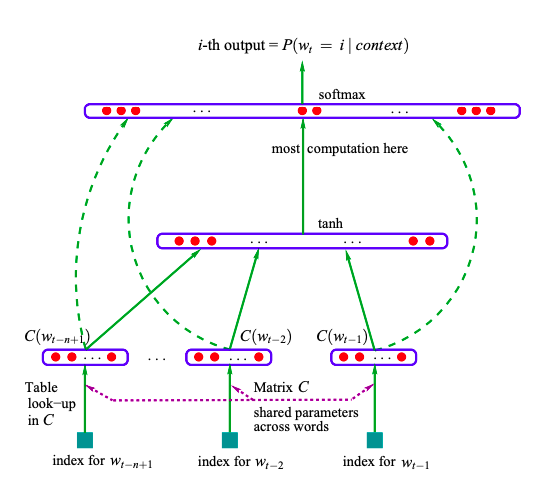
\includegraphics[scale = 0.8]{PNLM_architecture.png}
    \caption{Direct Architecture of Probabilistic Language Model}
    \label{fig:Probabilistic Language Model Architecture}
\end{figure}

The main result of this experiment is that the neural network performs much better than the smoothed trigram. Greater the length of the context words and higher the number of hidden units, the model becomes more efficient. Moreover, direct architecture was found to be better by about 2\% than the cycling architecture.

It can be deduced that the neural probabilistic model performs better due to the advantage of the learned distributed representation to fight the curse of dimensionality.